\subsection{Heading autopilot}\label{sec:prob1.1}
\subsubsection*{Analysis of ship characteristics}
To be able to model the ship in a good way we ran many simulations with different rudder angle and measured the steady-state yaw rate. We then made a $\delta-r$ plot of the result. Since the ship was turning port while giving a positive rudder command, this plot the rest of the assignment is made with a fixed gain of -1 on $\delta_c$.

\begin{figure}[h]
    \centering
    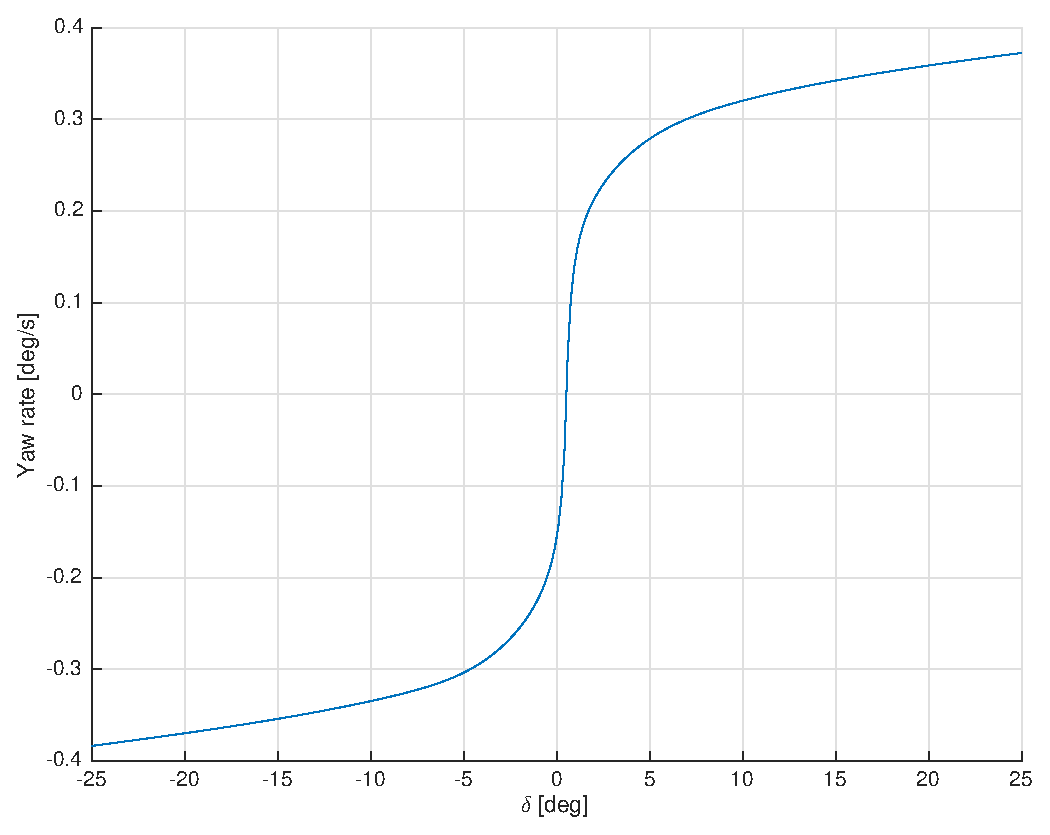
\includegraphics[width=\textwidth]{task1.4/Task1_4_delta_r_plot}
    \caption{$\delta - r$ plot}
    \label{fig:delta-r-plot}
\end{figure}

From figure \ref{fig:delta-r-plot} we clearly see the non-linear behavior of the ship. This motivates a 1-DOF heading model i.e. first- or second order Monoto model with non-linear extensions. To further investigate the effect of the non-linear characteristics of this ship, we compare the actual response with different models at different rudder angles. It should also be noticed that the ship has a constant drift to starboard with $\delta_c=0$, as seen by the curve not passing through the origin. We compensate for this through the rest of the modeling part by adding a fixed rudder angle of $0.52\degree$ to the rudder input. We only need this correction while estimating the model parameters. In a closed loop, the integral effect will cancel both this drift and drift caused by wind, current and waves.
\subsubsection*{1. order linear Nomoto}
As expected the first order Nomoto model will only be accurate for small rudder angles, and is therefore not very good for modeling the non-linearities. 
\begin{figure}[h]
    \centering
    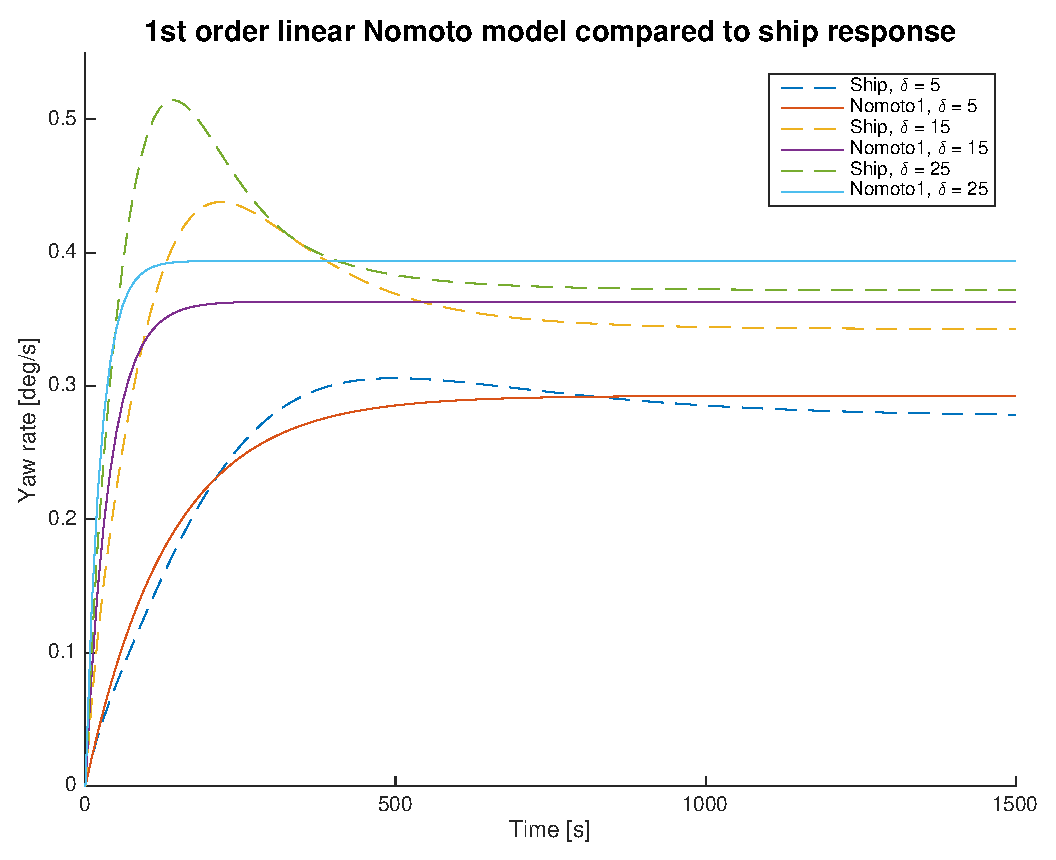
\includegraphics[width=\textwidth]{task1.4/Task1_4_Nomoto1}
    \caption{1.order linear Nomoto model}
    \label{fig:nomoto1}
\end{figure}

\subsubsection*{2. order linear Nomoto}
The second order Nomoto model follows the ship´s response much better, but...
\begin{figure}[h]
    \centering
    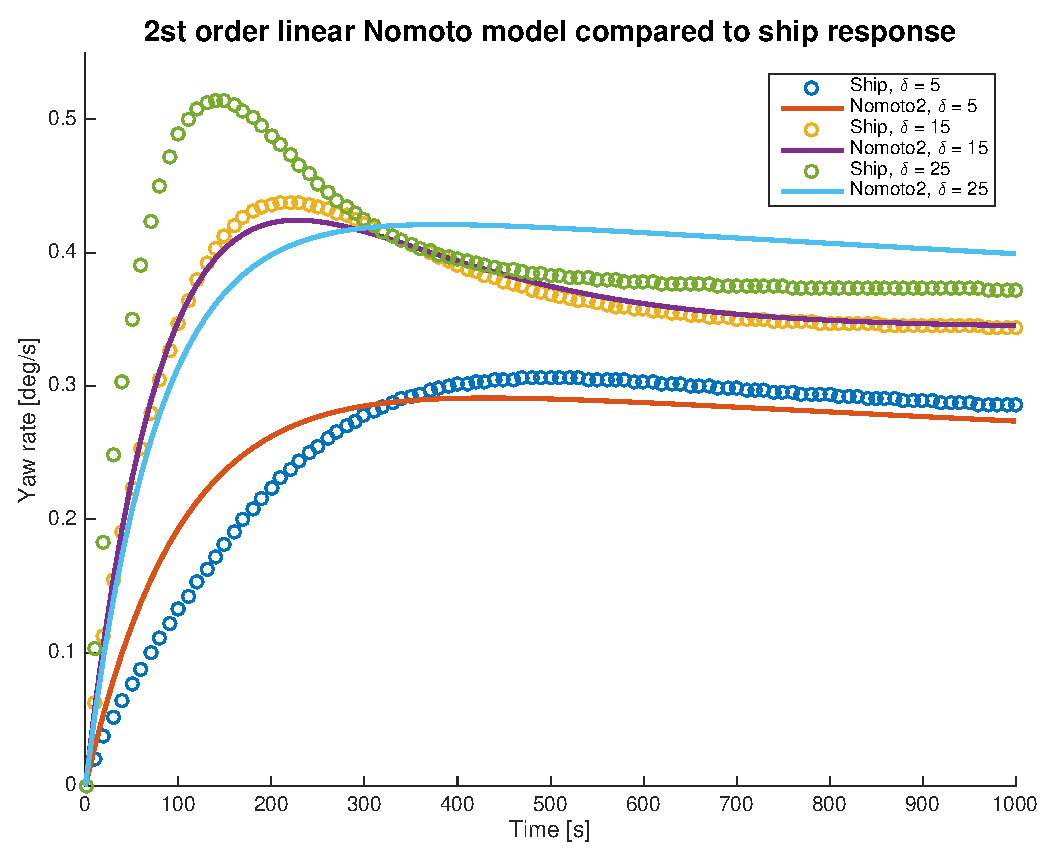
\includegraphics[width=\textwidth]{task1.4/Task1_4_Nomoto2}
    \caption{2.order linear Nomoto model}
    \label{fig:nomoto2}
\end{figure}


We model the heading of MS Fartøystyring with a Norrbin model
\begin{equation}
\begin{split}
\dot{\Psi} = r \\
T\dot{r}+n_3r^3 + n_1r=K\delta
\end{split}
\end{equation}
